\documentclass[12pt]{article}

\usepackage{amsmath}
\usepackage{amssymb}
\usepackage{geometry}
\usepackage{enumitem}
\usepackage{tikz}
\usetikzlibrary{
    arrows.meta,
    calc,
    angles,
    quotes,
    decorations.pathmorphing
}
\usepackage[american]{circuitikz}


\geometry{margin=1in}

\begin{document}

\begin{enumerate}[leftmargin=*]

 



\item In Young’s double slit experiment, slit separation is \(d=0.40\,\text{mm}\) and the screen is at \(D=1.5\,\text{m}\) using light of wavelength \(600\,\text{nm}\). A glass sheet of refractive index \(1.5\) and thickness \(3\,\mu\text{m}\) is inserted before one slit, introducing additional optical path difference while fringe width remains unchanged to first order. Determine the shift of the central maximum on the screen and identify the correct magnitude.  

% Q1
\begin{center}
\begin{tikzpicture}[scale=1]
\draw[thick] (0,1.5) -- (0,2.5);
\draw[thick] (0,-2.5) -- (0,-1.5);
\node[left] at (0,2) {$S_1$};
\node[left] at (0,-2) {$S_2$};

\draw[fill=gray!20] (0.05,1.6) rectangle (0.35,2.4);
\node at (0.2,2.6) {$\mu,t$};

\draw[thick] (7,-3) -- (7,3);
\node[right] at (7,0) {Screen};

\draw (0,2) -- (7,1);
\draw (0,-2) -- (7,-1);

\draw[<->] (0,-2.8) -- (0,-1.2);
\node[left] at (0,-2) {$d$};

\draw[<->] (0,-3.5) -- (7,-3.5);
\node at (3.5,-3.8) {$D$};
\end{tikzpicture}
\end{center}

A) \(5.63\,\text{mm}\)  

B) \(2.81\,\text{mm}\)  

C) \(1.41\,\text{mm}\)  

D) \(0.75\,\text{mm}\)  


\item A single slit of width \(0.20\,\text{mm}\) is illuminated by monochromatic light of wavelength \(500\,\text{nm}\), and a screen is placed \(2.0\,\text{m}\) away. Due to heating, the slit width decreases by \(5\%\) while wavelength remains constant, and small-angle approximation holds. Determine the new width of the central maximum on the screen including first-order correction.  

% Q2
\begin{center}
\begin{tikzpicture}[scale=1]
\draw[thick] (0,-1) -- (0,1);
\node[left] at (0,0) {Slit};

\draw[thick] (6,-2.5) -- (6,2.5);
\node[right] at (6,0) {Screen};

\draw[dashed] (0,0) -- (6,0);

\draw (0,1) -- (6,1.5);
\draw (0,-1) -- (6,-1.5);

\draw[<->] (-0.5,-1) -- (-0.5,1);
\node[left] at (-0.5,0) {$a$};
\end{tikzpicture}
\end{center}

A) \(1.05\,\text{cm}\)  

B) \(1.00\,\text{cm}\)  

C) \(0.95\,\text{cm}\)  

D) \(1.10\,\text{cm}\)  


\item Light of frequency \(1.2\times10^{15}\,\text{Hz}\) is incident on a metal with work function \(2.0\,\text{eV}\). The frequency is reduced by \(5\%\) while intensity is doubled, but emission remains in linear regime and relativistic corrections are negligible. Determine the new stopping potential considering only first-order change in photon energy.  

A) \(2.76\,\text{V}\)  

B) \(2.97\,\text{V}\)  

C) \(3.10\,\text{V}\)  

D) \(2.50\,\text{V}\)  


\item An electron accelerated through \(150\,\text{V}\) enters a uniform magnetic field perpendicular to its velocity and moves in a circular path. The accelerating voltage decreases by \(2\%\) while magnetic field increases by \(4\%\), and non-relativistic approximation is valid. Determine the fractional change in radius of the circular path to first order.  

% Q4
\begin{center}
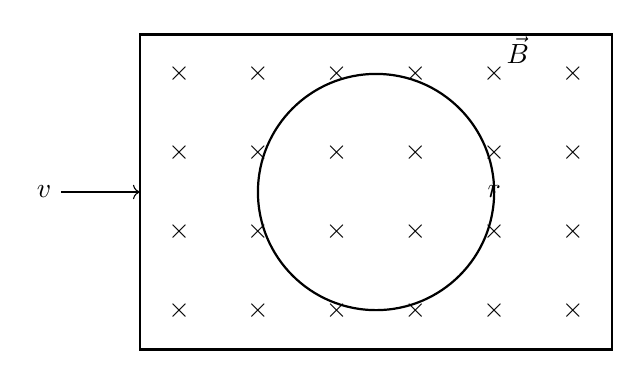
\begin{tikzpicture}[scale=1]
\draw[thick] (-1,-2) rectangle (5,2);

\foreach \x in {-0.5,0.5,...,4.5}
  \foreach \y in {-1.5,-0.5,0.5,1.5}
    \node at (\x,\y) {$\times$};

\node at (3.8,1.8) {$\vec{B}$};

\draw[thick] (2,0) circle (1.5);
\node at (3.5,0) {$r$};

\draw[->] (-2,0) -- (-1,0);
\node[left] at (-2,0) {$v$};
\end{tikzpicture}
\end{center}

A) Radius decreases by \(6\%\)  

B) Radius decreases by \(3\%\)  

C) Radius unchanged  

D) Radius increases by \(2\%\)  


\item A radioactive sample initially contains \(10^{20}\) nuclei and after \(40\) days only \(1/16\) remains, following ideal exponential decay. During measurement the detector efficiency drops by \(10\%\), but decay law itself is unaffected. Determine the true half-life of the sample.  

A) \(10\,\text{days}\)  

B) \(8\,\text{days}\)  

C) \(12\,\text{days}\)  

D) \(20\,\text{days}\)  


\item In the Bohr model of hydrogen, an electron transitions from \(n=4\) to \(n=2\) and the nucleus mass is considered finite using reduced mass correction to first order in \(m_e/m_p\). The Rydberg constant effectively modifies due to this correction while selection rules remain unchanged. Determine the corrected wavelength expression and identify the spectral series.  

% Q6
\begin{center}
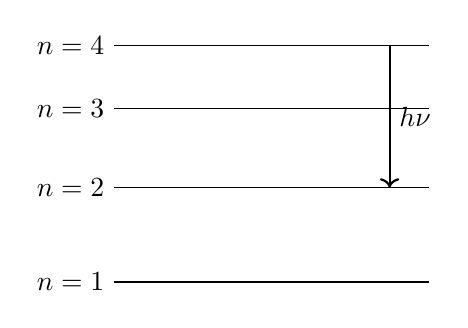
\begin{tikzpicture}[scale=1]
\draw (0,0) -- (4,0);
\draw (0,1.2) -- (4,1.2);
\draw (0,2.2) -- (4,2.2);
\draw (0,3) -- (4,3);

\node[left] at (0,0) {$n=1$};
\node[left] at (0,1.2) {$n=2$};
\node[left] at (0,2.2) {$n=3$};
\node[left] at (0,3) {$n=4$};

\draw[->,thick] (3.5,3) -- (3.5,1.2);
\node[right] at (3.5,2.1) {$h\nu$};
\end{tikzpicture}
\end{center}

A) \(\dfrac{16}{3R}\left(1+\dfrac{m_e}{m_p}\right)\), Balmer  

B) \(\dfrac{16}{3R}\left(1-\dfrac{m_e}{m_p}\right)\), Balmer  

C) \(\dfrac{4}{3R}\left(1-\dfrac{m_e}{m_p}\right)\), Lyman  

D) \(\dfrac{16}{5R}\left(1-\dfrac{m_e}{m_p}\right)\), Paschen  


\item A PN junction diode operates at \(300\,\text{K}\) with forward current proportional to \(e^{eV/kT}\). The forward bias increases by \(60\,\text{mV}\) while temperature rises by \(5\%\), and ideal diode equation remains valid. Determine the multiplicative change in current to first order accuracy.  

A) \(\times 8\)  

B) \(\times 10\)  

C) \(\times 6\)  

D) \(\times 12\)  


\item An optical fibre has core refractive index \(1.50\) and cladding index \(1.40\), and both decrease uniformly by \(0.01\) due to temperature rise. The difference in refractive index remains unchanged to first order and light is incident from air. Determine the new numerical aperture.  

A) \(0.54\)  

B) \(0.40\)  

C) \(0.36\)  

D) \(0.30\)  


\item An electron and a proton possess equal kinetic energy \(K\) under non-relativistic conditions. The proton kinetic energy increases by \(1\%\) while the electron kinetic energy decreases by \(1\%\), and de Broglie relation remains valid. Determine the ratio of their de Broglie wavelengths including first-order correction.  

A) \(\sqrt{\dfrac{m_p}{m_e}}\left(1-0.01\right)\)  

B) \(\sqrt{\dfrac{m_p}{m_e}}\left(1+0.01\right)\)  

C) \(\sqrt{\dfrac{m_e}{m_p}}\left(1-0.01\right)\)  

D) \(\sqrt{\dfrac{m_p}{m_e}}\)  


\item In Young’s experiment fringe width is given by \(\beta=\lambda D/d\). The slit separation doubles, wavelength halves, and screen distance increases by \(10\%\) simultaneously under small-angle approximation. Determine the new fringe width in terms of initial \(\beta_0\).  

A) \(0.275\,\beta_0\)  

B) \(0.25\,\beta_0\)  

C) \(0.50\,\beta_0\)  

D) \(0.125\,\beta_0\)  


\item In photoelectric effect, when frequency is increased slightly above threshold while intensity is decreased such that total power remains constant, the stopping potential changes. This occurs because maximum kinetic energy depends only on photon energy difference from threshold.  

A) \(h(\nu-\nu_0)\)  

B) Intensity  

C) Photon momentum  

D) Surface area  


\item In single slit diffraction, intensity of secondary maxima decreases rapidly with angle although total energy is conserved. This is because amplitude contributions from different parts of slit undergo varying phase differences producing progressive cancellation.  

A) Destructive phase variation across slit  

B) Energy absorption  

C) Reduced wavelength  

D) Photon loss  


\item In intrinsic semiconductor, conductivity varies with temperature as \(\sigma \propto e^{-E_g/2kT}\) multiplied by mobility factor that slightly decreases with temperature. For small rise in temperature, the exponential increase in carrier concentration dominates mobility decrease.  

A) Thermal excitation across band gap  

B) Reduced mobility  

C) Increased resistance  

D) Decreased band gap only  


\item The binding energy per nucleon curve rises sharply for light nuclei and peaks near iron. Fusion of two light nuclei releases energy because the resulting nucleus has higher average binding energy per nucleon and lower mass defect per nucleon ratio.  

A) Higher binding energy per nucleon  

B) Lower binding energy  

C) Constant binding energy  

D) Zero binding energy  


\item In an optical fibre, total internal reflection occurs when angle of incidence exceeds the critical angle determined by refractive indices. Under this condition, the wave in cladding has an evanescent character while propagation continues along the fibre axis.  

% Q15
\begin{center}
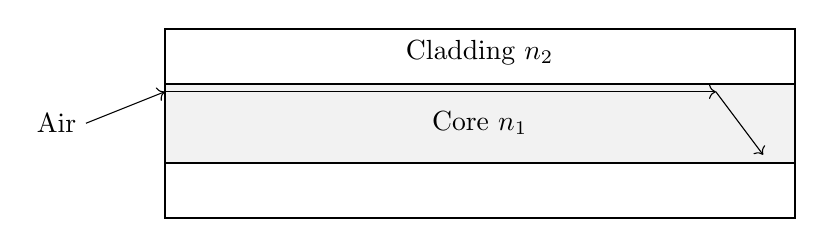
\begin{tikzpicture}[scale=1]

% Cladding (outer region)
\draw[thick] (-4,-1.2) rectangle (4,1.2);

% Core (inner region)
\draw[thick, fill=gray!10] (-4,-0.5) rectangle (4,0.5);

% Labels
\node at (0,0) {Core $n_1$};
\node at (0,0.9) {Cladding $n_2$};

% Incident ray from air
\draw[->] (-5,0) -- (-4,0.4);
\node[left] at (-5,0) {Air};

% Ray inside core
\draw[->] (-4,0.4) -- (3,0.4);

% Reflected ray
\draw[->] (3,0.4) -- (3.6,-0.4);

\end{tikzpicture}
\end{center}

A) Imaginary transverse component in cladding  

B) Zero wave vector  

C) Equal propagation constants  

D) Complete absorption  


\end{enumerate}

\end{document}